
\documentclass[a4paper,11pt]{report}
\usepackage[]{graphicx}
\usepackage[]{color}
%% maxwidth is the original width if it is less than linewidth
%% otherwise use linewidth (to make sure the graphics do not exceed the margin)
\makeatletter

\usepackage{geometry}
\geometry{verbose,tmargin=2cm,bmargin=2cm,lmargin=2cm,rmargin=2cm}
\usepackage{enumerate}
\usepackage[T1]{fontenc}      
\usepackage[utf8]{inputenc} 
\usepackage[francais]{babel}  
\usepackage{fancyhdr}
\usepackage{graphicx}
\usepackage{amssymb}
\usepackage{amsmath}
\usepackage{tikz}
\usepackage{parskip}
\usepackage{listings}
\pagestyle{fancy}
\selectlanguage{francais}
\linespread{1.1}

\newcounter{numero}
\newcommand{\exo}{
	{\large
		\vspace{5mm}
		\addtocounter{numero}{1}
		{\bf Problème~\thenumero}
		\vspace{2mm}
	}
}
\newcommand{\tab}{\hspace{1em}}

\fancyhead[L]{\footnotesize SIO - TP1}
\fancyfoot[C]{\thepage} 
\thispagestyle{empty} % Pour ne pas avoir de header/footer sur la première page

\begin{document}
	
{\sc HEIG--VD} \hfill Bastien Clément\newline 
Simulation et Optimisation \hfill \today \newline
\hrule
\vspace{2mm}
{\large \bf Rapport~: Génération de variables aléatoires} \hfill {\large \bf Travail personnel~1}
\vspace{4mm}
\hrule

\exo
\begin{enumerate}[\indent a)]\itemsep3mm\topsep0mm
	
\item {\em Donner une définition par morceaux de $\tilde{f}(x)$.}

\begin{equation*}
\tilde{f}(x) = \left\lbrace \begin{array}{ll}
	0						& \text{si $x < x_0$} \\
	m_0 ( x - x_0 ) + y_0	& \text{si $x_0 \leq x \leq x_1$} \\
	0 						& \text{si $x > x_1$}
\end{array} \right.
\end{equation*}

Avec $x_0 < x_1$; $y_0, y_1 \in \mathbb{R}^{+}$ et $m_0 = \frac{y_1-y_0}{x_1-x_0}$.

\item {\em On désire définir une variable aléatoire $X$ de densité $f(x)$ proportionnelle à $\tilde{f}(x)$. Déterminer la constante de proportionnalité, c.à-d. déterminer la constante $A_{0}$ telle que $f(x) = \frac{1}{A_{0}}\tilde{f}(x)$ soit une densité.}

Puisque $A_{0}$ est une constante et que $f(x)$ est une densité, nous savons que
\begin{equation*}
	\int_{-\infty}^{\infty} f(x)\,dx =
	\int_{x_0}^{x_1} \frac{1}{A_0} \tilde{f}(x)\,dx =
	\frac{1}{A_0} \int_{x_0}^{x_1} \tilde{f}(x)\,dx = 1
\end{equation*}

Il n'est pas nécessaire de considérer les cas $x < x_0$ et $x > x_1$ puisque la fonction est nulle en dehors de l'intervalle $[x_0; x_1]$. Il alors est évident que
\begin{equation*}
	A_0 = \int_{x_0}^{x_1} \tilde{f}(x)dx
\end{equation*}

c'est à dire l'aire sous la courbe de $\tilde{f}(x)$ sur l'intervalle $[x_0; x_1]$. Dans notre cas, le problème est simplifié puisque nous avons un trapèze rectangle dont l'aire est donnée par le produit de la base moyenne et de la hauteur:
\begin{equation*}
	A_0 = \frac{y_0 + y_0}{2} \cdot (x_1 - x_0).
\end{equation*}

Nous pouvons finalement définir
\begin{align*}
	f(x) &= \frac{1}{A_0} \cdot  \tilde{f}(x) \\
	     &= \frac{2}{(y_0 + y_1)(x_1 - x_0)} \cdot \tilde{f}(x)
\end{align*}

\item {\em Calculer l'espérance de la variable $X$, sans oublier de simplifier votre résultat.}

L'espérance mathématique d'une variable aléatoire est définie par
\begin{equation*}
	\mathbb{E}[x] = \int_{-\infty}^{\infty} x f(x) \,dx
\end{equation*}

Dans notre cas, nous pouvons à nouveau nous limiter à l'intervalle $[x_{0}; x_{1}]$ puisque en dehors de cet intervalle, $f(x)=0$.

Nous avons donc:
\begingroup
\addtolength{\jot}{1em}
\begin{align*}
\mathbb{E}[x] &= \int_{x_0}^{x_1} x f(x) \,dx \\
	&= \frac{1}{A_0} \int_{x_0}^{x_1} x \tilde{f}(x) \,dx \\
	&= \frac{2}{(y_0 + y_1)(x_1 - x_0)} \cdot \int_{x_0}^{x_1} x (m_0 \cdot (x - x_0) + y_0) \,dx \\
	&= \frac{2}{(y_0 + y_1)(x_1 - x_0)} \cdot \left( \frac{x^2 \big(2x (y_0-y_1) + 3 x_0 y_1 - 3 x_1 y_0\big)}{6 (x_0-x_1)}+c \biggr\rvert^{x_1}_{x_0} \right) \\
	&= \frac{2}{(y_0 + y_1)(x_1 - x_0)} \cdot \frac{\big(x_1-x_0\big) \big(x_0 (2 y_0+y_1)+x_1 (y_0+2 y_1)\big)}{6} \\
	&= \frac{x_0 (2y_0 + y_1) + x_1 (y_0 + 2y_1)}{3 (y_0+y_1)}
\end{align*}
\endgroup

\item {\em Vérifier que, dans le cas où $y_{0} \neq y_{1}$, la fonction de répartition de la variable $X$ est}
\begin{equation*}
	F(x) = P(X \leq x) = \left\lbrace \begin{array}{ll}
		0						& \text{si $x < x_0$} \\
		\frac{1}{y^2_1 - y^2_0} \left( \left( m_0 \left( x - x_0 \right) + y_0 \right)^2 - y^2_0 \right)	& \text{si $x_0 \leq x \leq x_0$} \\
		1 						& \text{si $x > x_1$}
	\end{array} \right.
\end{equation*}

{\em Le développement du point d) n'est pas demandé. }

\item {\em Utiliser le résultat précédent pour proposer un algorithme permettant de générer des réalisations de la variable $X$ à l'aide de la méthode des fonctions inverses. Traiter séparément les cas $y_{0} = y_{1}$ et $y_{0} \neq y_{1}$.}

Notre fonction de répartition $F(x)$, liée à la fonction de densité $f(x)$, est définie comme une fonction $\mathbb{R} \rightarrow [0;1]$ mais en pratique, le domaine intéressant se limite à $[x_0;x_1]$ puisque que
\begin{align*}
	x < x_0 &\implies F(X) = 0 \\
	x > x_1 &\implies F(X) = 1
\end{align*}

\begin{center}
	\begin{tabular}{cc}
		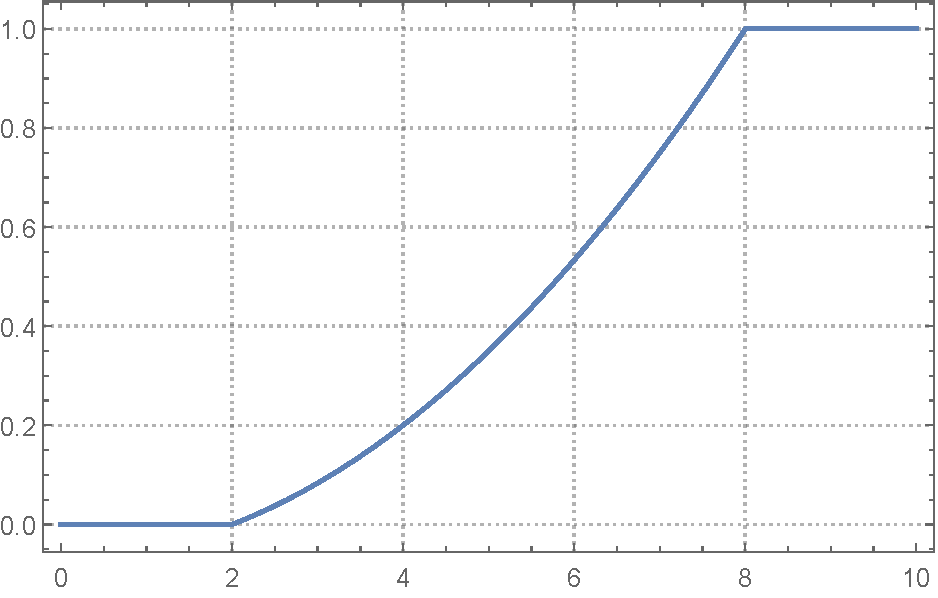
\includegraphics[width=7cm]{img_graph2} & 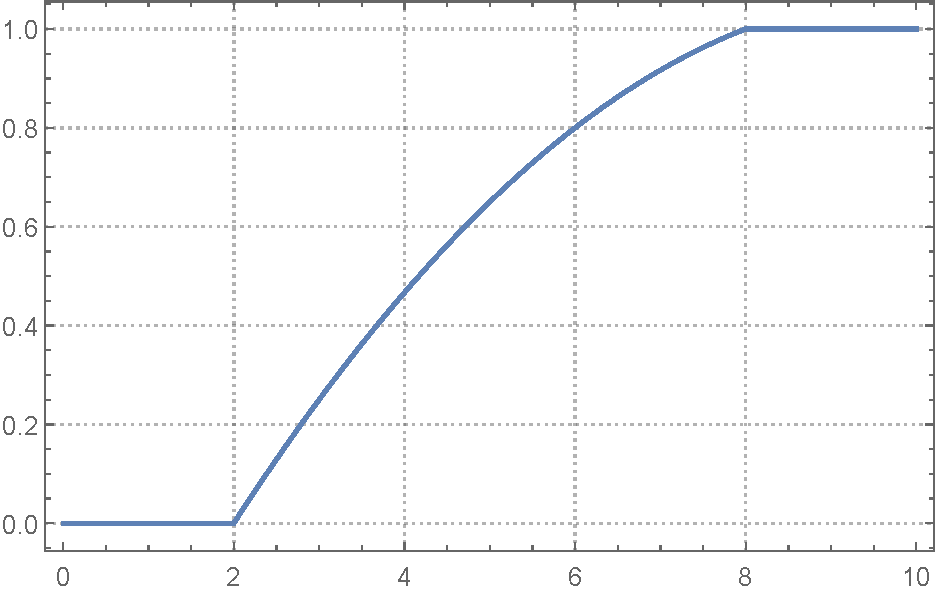
\includegraphics[width=7cm]{img_graph1} \\
		{\footnotesize Exemple de graphe pour $F(x)$ avec $y_0 < y_1$} & {\footnotesize Exemple de graphe pour $F(x)$ avec $y_0 > y_1$}
	\end{tabular}
\end{center}

La méthode des fonctions inverses consiste à utiliser la réciproque  $F^{-1}(y) : [0;1] \rightarrow [x_0;x_1]$ et une variable $y \sim \mathcal{U}(0, 1)$ pour déterminer une réalisation $x = F^{-1}(y)$ conforme à la densité de probabilité désirée pour $X$.

Inversion de $y = F(x) \mid x \in [x_0, x_1], y_0 \ne y_1$:
\begingroup
\addtolength{\jot}{1em}
\begin{align*}
	y &= \frac{1}{y^2_1 - y^2_0} \cdot \left( \left( m_0 \cdot  \left( x - x_0 \right) + y_0 \right)^2 - y^2_0 \right) \\
	y \cdot (y_1^2 - y_0^2) + y^2_0 &=  \left( m_0 \cdot  \left( x - x_0 \right) + y_0 \right)^2\\
	\pm \sqrt{y \cdot (y_1^2 - y_0^2) + y^2_0} &=  m_0 \cdot  \left( x - x_0 \right) + y_0 \\
	\frac{\pm \sqrt{y \cdot (y_1^2 - y_0^2) + y^2_0} - y_0}{m_0} + x_0 &=  x
\end{align*}
\endgroup

Dans le cas où $y_1 = y_0$, la solution est simple: la densité de probabilité définie par $f$ est une uniforme sur l'intervalle $[x_0;x_1]$ que l'on peut générer très facilement à partir d'une uniforme sur l'intervalle $[0,1]$.
\begin{equation*}
	u \sim \mathcal{U}(a,b) = a + (b - a) \big( v \sim \mathcal{U}(0, 1) \big)
\end{equation*}

Dans le cas contraire, nous devons déterminer le signe de la racine. En observant les graphes de la fonction $F(x)$ pour $y_0 < y_1$ et $y_0 > y_1$, on en déduit assez facilement que le signe dépend de la relation entre $y_0$ et $y_1$. Nous pouvons alors définir:
\begin{equation*}
	F^{-1}(y): [0;1] \rightarrow [x_0,x_1] = \left\lbrace \begin{array}{ll}
		x_0 + \frac{- y_0 + \sqrt{y \cdot (y_1^2 - y_0^2) + y^2_0}}{m_0}
		& \text{si $y_0 < y_1$} \\
		x_0 + y \cdot (x_1 - x_0)
		& \text{si $y_0 = y_1$} \\
		x_0 + \frac{- y_0 - \sqrt{y \cdot (y_1^2 - y_0^2) + y^2_0}}{m_0}
		& \text{si $y_0 > y_1$} \\
	\end{array} \right.
\end{equation*}

L'algorithme de génération de réalisations est alors trivial:
\begin{enumerate}[1]
	\ttfamily
	\item Générer $y \sim \mathcal{U}(0, 1)$
	\item Retourner $F^{-1}(y)$
\end{enumerate}

\item {\em Développer un algorithme permettant de générer des réalisations de la variable $X$ à l'aide d'une approche géométrique basée sur la méthode d'acceptation-rejet et en utilisant efficacement les symétries.}

La méthode d'acceptation-rejet consiste à \emph{enfermer} notre fonction de densité $f(x)$ sous une fonction de densité $g(x)$ plus simple tel que $\forall x \in [x_0,x_1], f(x) \leq c \cdot g(x) \mid c \in \mathbb{R}$ pour laquelle nous savons générer des réalisations aléatoires. Nous retournerons alors des réalisations $y \sim g$ si $\mathcal{U}(0,1) \leq \frac{f(y)}{cg(y)}$.

Dans notre cas, il n'est même pas nécessaire de respecter strictement le concept de fonction de densité et nous pouvons utiliser directement $\tilde{f}$, dont le maximum $y_m = \textnormal{max}(y_0, y_1)$ et générer des réalisations $(a,b) \mid a \sim \mathcal{U}(x_0, x_1), b \sim \mathcal{U}(0, y_m)$ qui correspondent à des points uniformément distribués dans le rectangle sous la courbe de la fonction $g(x)=y_m$ sur l'intervalle $[x_0, x_1]$.

\begin{center}
	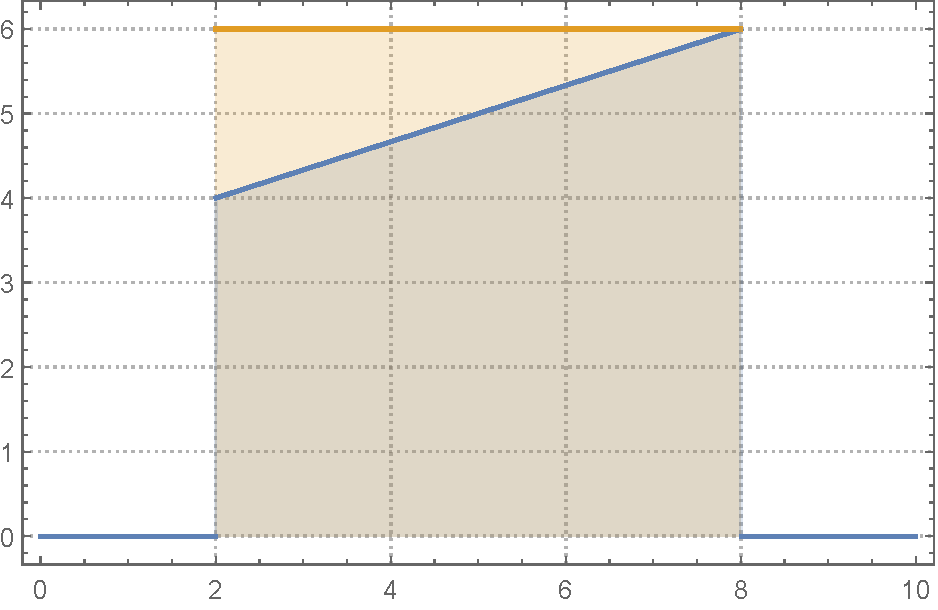
\includegraphics[width=8cm]{img_graph3}\\
	{\footnotesize Graphe de $\tilde{f}(x) = \left\lbrace \begin{array}{ll}
		\frac{1}{3} ( x - 2 ) + 4 & \text{si $2 \leq x \leq 8$} \\
		0 						& \text{sinon}
		\end{array} \right.$ et $g(x)=y_m=6$}
\end{center}

Nous retournerons alors $a$ si $b \leq \tilde{f}(a)$ est vérifié. Dans le cas contraire, de nouvelles réalisations de $a$ et $b$ devront être générées jusqu'à vérifier l'inégalité.

Cependant, puisque le segment $\big\lbrace (x_0,y_0) , (x_1,y_1) \big\rbrace$ délimitant l'aire de $\tilde{f}$ est une diagonale du rectangle $\big\lbrace (x_0,y_0) , (x_1,y_0) , (x_1,y_1) , (x_0,y_1) \big\rbrace$, il est possible de \emph{rattraper le coup} lorsque le point $(a,b)$ est en dehors de l'aire de $\tilde{f}$ en effectuant une symétrie par rapport au centre du rectangle pour déplacer un point tombé dans le mauvais triangle dans le bon triangle.

\begin{center}
	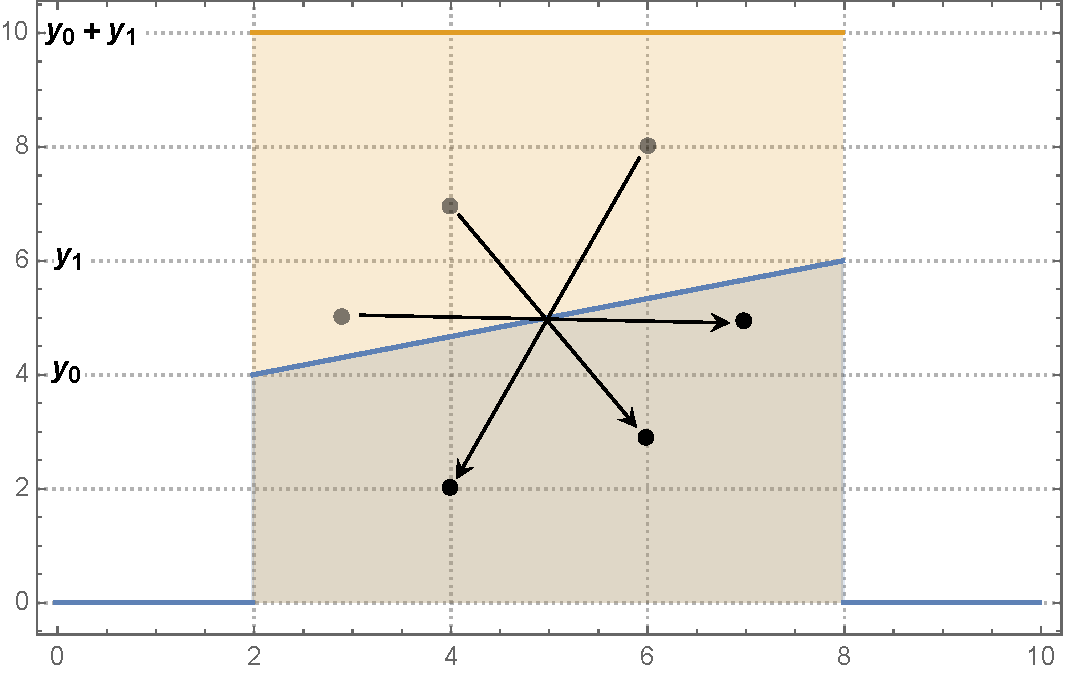
\includegraphics[width=8cm]{img_graph4}\\
	{\footnotesize Récupération de points dans le mauvais triangle}
\end{center}

Nous avons donc l'algorithme suivant, sans possibilité de rejet:
\begin{enumerate}[1]
	\ttfamily
	\item Définir $y_m = \textnormal{max}(y_0, y_1)$
	\item Générer $a \sim \mathcal{U}(x_0,x_1)$ et $b \sim \mathcal{U}(0,y_m)$
	\item Si $b \leq \tilde{f}(a)$ alors
	\item \tab // Dans l'aire de $\tilde{f}(x)$
	\item \tab Retourner $a$
	\item Sinon
	\item \tab // Hors de l'aire de $\tilde{f}(x)$, on prend la symétrie
	\item \tab Retourner $x_1 - (a - x_0)$
	\item Fin
\end{enumerate}

\end{enumerate}

\exo
\begin{enumerate}[\indent a)]\itemsep3mm\topsep2mm
	
\item {\em Déterminer la constante $A$ telle que $f=\frac{1}{A}\tilde{f}$ soit une densité}

\item {\em Développer un algorithme pour générer des réalisations de la variable $X$ basé sur une application directe, "bête et méchante", de la méthode d'acceptation-rejet.}

\item {\em Développer un algorithme pour générer des réalisations de la variable $X$ basé sur la méthode des mélanges et sur la méthode développée au point f) du problème précédent.}

\end{enumerate}


\end{document}